%To compile as handout, use
%pdflatex "\def\ishandout{1} \input{filename.tex}"
%Defaults to non-handout mode (with slide reveals)
\ifdefined\ishandout
  \documentclass[handout]{beamer}
\else
  \documentclass{beamer}
\fi
 
\usepackage{econ103slides} 

\date{Lecture \# 3}
\begin{document} 




%%%%%%%%%%%%%%%%%%%%%%%%%%%%%%%%%%%%%%%%

\begin{frame}[plain]
	\titlepage 
	

\end{frame} 

%%%%%%%%%%%%%%%%%%%%%%%%%%%%%%%%%%%%%%%%
\begin{frame}
\frametitle{Recall From Last Lecture: }

\begin{block}{Range}
Maximum Observation - Minimum Observation
\end{block}

\begin{block}{Interquartile Range (IQR)}
IQR= $\mbox{Q}_3 - \mbox{Q}_1$
\end{block}

\begin{block}{Variance}
$\displaystyle s^2 = \frac{1}{n-1} \sum_{i=1}^n (x_i - \bar{x})^2$
\end{block}

 \begin{block}{Standard Deviation}
	$s = \sqrt{s^2}$
\end{block}
\end{frame}
%%%%%%%%%%%%%%%%%%%%%%%%%%%%%%%%%%%%%%%%

\begin{frame}
\frametitle{Recall From Last Lecture:}
\begin{block}{Variance}
Essentially the average squared distance from the mean. Sensitive to both skewness and outliers.
\end{block}

\begin{block}{Standard Deviation}
$\sqrt{\mbox{Variance}}$, but more convenient since \alert{same units as data}
\end{block}

\begin{block}{Range}
Difference between larges and smallest observations. \emph{Very} sensitive to outliers. Displayed in boxplot.
\end{block}

\begin{block}{Interquartile Range}
Range of middle 50\% of the data. Insensitive to outliers, skewness. Displayed in boxplot.
\end{block}

\end{frame}


%%%%%%%%%%%%%%%%%%%%%%%%%%%%%%%%%%%%%%%%
\begin{frame}
\frametitle{Why Squares?}
\begin{center}\fbox{$\displaystyle s^2 = \frac{1}{n-1}\sum_{i=1}^n(x_i - \bar{x})^2$}\end{center}
\begin{alertblock}{What's Wrong With This?}
	\begin{eqnarray*}
		\displaystyle\frac{1}{n-1}\sum_{i=1}^N (x_i - \bar{x}) &=& \pause\frac{1}{n-1}\left[\sum_{i=1}^n x_i - \sum_{i=1}^n \bar{x} \right] = \pause\frac{1}{n-1}\left[ \sum_{i=1}^n x_i  - n\bar{x}\right]\\
			&=& \pause \frac{1}{n-1}\left[ \sum_{i=1}^n x_i  - n\cdot\frac{1}{n} \sum_{i=1}^n x_i\right]\\ &=& \pause \frac{1}{n-1}\left[ \sum_{i=1}^n x_i  -  \sum_{i=1}^n x_i\right] =\pause 0
	\end{eqnarray*}
\end{alertblock}

\end{frame}
%%%%%%%%%%%%%%%%%%%%%%%%%%%%%%%%%%%%%%%%

\begin{frame}
\frametitle{Variance is Sensitive to Skewness and Outliers}
\framesubtitle{And so is Standard Deviation!}
\begin{center}\fbox{$\displaystyle s^2 = \frac{1}{n-1}\sum_{i=1}^n(x_i - \bar{x})^2$}\end{center}


\begin{block}{Outliers}
Differentiate with respect to $(x_i-\bar{x})\Rightarrow$ the farther an observation is from the mean, the \emph{larger} its effect on the variance.
\end{block}


\begin{block}{Skewness}
Variance measures average squared distance from center, taking \alert{mean} as the center, but the mean is sensitive to skewness!
\end{block}

\end{frame}

%%%%%%%%%%%%%%%%%%%%%%%%%%%%%%%%%%%%%%%%
\begin{frame}

\frametitle{Skewness -- A Measure of Symmetry}

\begin{center}
\fbox{$\displaystyle\mbox{Skewness} = \frac{1}{n}\frac{\sum_{i=1}^n (x_i - \bar{x})^3}{s^3}$}
\end{center}
\pause
\begin{block}{What do the values indicate?}Zero $\Rightarrow$ symmetry, positive right-skewed, negative left-skewed.\end{block} \pause
\begin{block}{Why cubed?}To get the desired sign.\end{block} \pause
\begin{block}{Why divide by $s^3$?}So that skewness is unitless\end{block}\pause
\begin{block}{Rule of Thumb}Typically (but not always), right-skewed $\Rightarrow$ mean $>$ median\\ left-skewed $\Rightarrow$ mean $<$ median\end{block}

\end{frame}


%%%%%%%%%%%%%%%%%%%%%%%%%%%%%%%%%%%%%%%%


\begin{frame}
\centering 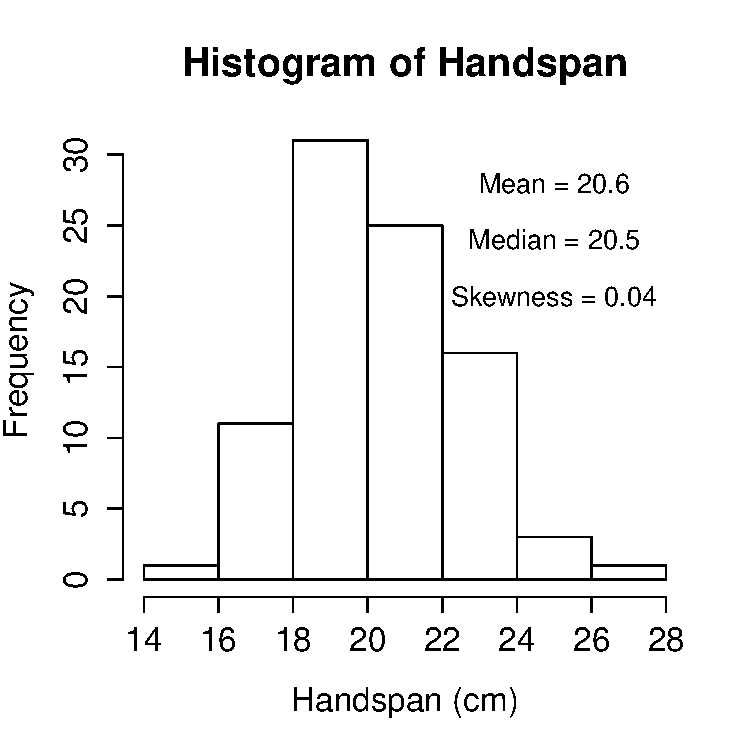
\includegraphics[scale = 0.75]{./images/handspan_skew}


\end{frame}

%%%%%%%%%%%%%%%%%%%%%%%%%%%%%%%%%%%%%%%%


\begin{frame}
\centering 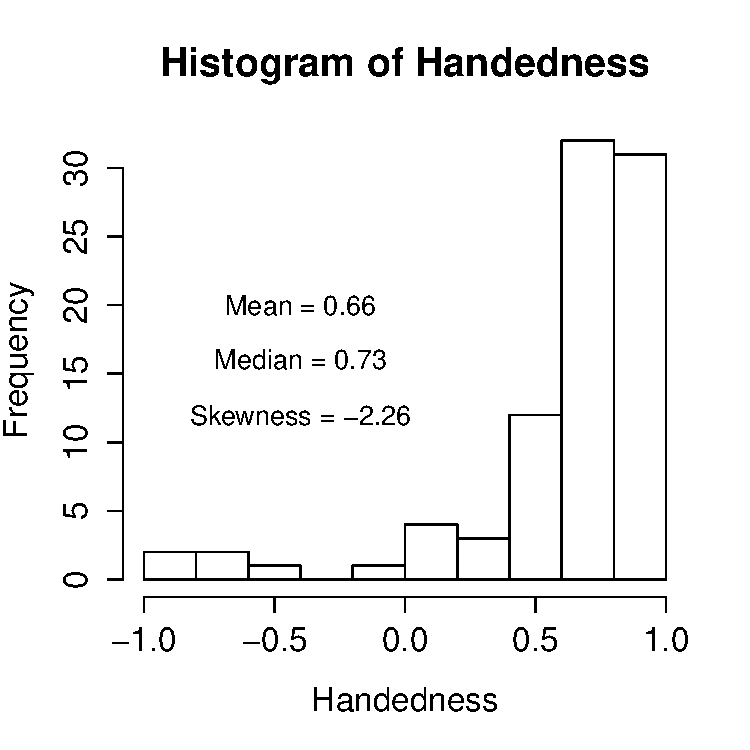
\includegraphics[scale = 0.75]{./images/handedness_skew}


\end{frame}
%%%%%%%%%%%%%%%%%%%%%%%%%%%%%%%%%%%%%%%%
\begin{frame}
\frametitle{Essential Distinction: Sample vs.\ Population}
For now, you can think of the population as a list of $N$ objects:\\
	\alert{$\mbox{Population: }x_1, x_2, \hdots, x_N$}\\
from which we draw a sample of size $n<N$ objects:\\
	\alert{$\mbox{Sample: } x_1, x_2, \hdots, x_n$}
\pause
\vspace{3em}
\begin{alertblock}{Important Point:}
Later in the course we'll be more formal by considering \alert{probability models} that represent the \alert{\emph{act of sampling}} from a population rather than thinking of a population as a list of objects. Once we do this we will no longer use the notation $N$ as the population will be \alert{\emph{conceptually infinite}}.
\end{alertblock}
\end{frame}

%%%%%%%%%%%%%%%%%%%%%%%%%%%%%%%%%%%%%%%%
\begin{frame}

\frametitle{Essential Distinction: Parameter vs.\ Statistic}
$N$ individuals in the Population, $n$ individuals in the Sample:

\vspace{1em}
\small
\begin{tabular}{l|l|l}
	&\textbf{Parameter} (Population)&\textbf{Statistic} (Sample)\\
	\hline
	Mean&$\displaystyle\mu = \frac{1}{N} \sum_{i=1}^N x_i$& $\displaystyle\bar{x} = \frac{1}{n} \sum_{i=1}^n x_i$ \\
	Var.\ &$\displaystyle \sigma^2 = \frac{1}{N}\sum_{i=1}^N (x_i - \mu)^2$ &$\displaystyle s^2 = \frac{1}{n-1}\sum_{i=1}^n(x_i - \bar{x})^2$\\
	S.D.\ &$\sigma = \sqrt{\sigma^2}$ &$s = \sqrt{s^2}$ \\
	&&
\end{tabular}

\vspace{2em}
\begin{alertblock}{Key Point}
We  use a \alert{sample} $x_1, \hdots, x_n$ to calculate \alert{statistics} (e.g.\ $\bar{x}$, $s^2$, $s$) that serve as \alert{estimates} of the corresponding population \alert{parameters} (e.g.\ $\mu$, $\sigma^2$, $\sigma$).
\end{alertblock}
\end{frame}
%%%%%%%%%%%%%%%%%%%%%%%%%%%%%%%%%%%%%%%%
\begin{frame}
\frametitle{Why Do Sample Variance and Std.\ Dev.\ Divide by $n-1$? }
\footnotesize
\fbox{\begin{tabular}{ll|ll}
Pop.\ Var.\ &$\displaystyle \sigma^2 = \frac{1}{N}\sum_{i=1}^N (x_i - \mu)^2$&Sample Var.\ &$\displaystyle s^2 = \frac{1}{n-1}\sum_{i=1}^n(x_i - \bar{x})^2$\\
\hline
Pop.\ S.D.\ &$\sigma = \sqrt{\sigma^2}$ &Sample S.D.\ &$s = \sqrt{s^2}$ \\
\end{tabular}}
\normalsize

\vspace{3em}
\alert{There is an important reason for this, but explaining it requires some concepts we haven't learned yet. }

\end{frame}


%%%%%%%%%%%%%%%%%%%%%%%%%%%%%%%%%%%%%%%%
\begin{frame}
\frametitle{Why Mean and Variance (and Std.\ Dev.\ )?}
\begin{alertblock}{Empirical Rule}
For large populations that are approximately bell-shaped, std.\ dev.\ tells where most observations will be relative to the mean:
	\begin{itemize}
		\item $\approx$ 68\% of observations are in the interval $\mu \pm \sigma$
		\item $\approx$ 95\% of observations are in the interval $\mu \pm 2\sigma$
		\item Almost all of observations are in the interval $\mu \pm 3\sigma$
	\end{itemize}
\end{alertblock}
\pause

\begin{block}{Therefore}
We will be interested in $\bar{x}$ as an estimate of $\mu$ and $s$ as an estimate of $\sigma$ since these population parameters are so informative.
\end{block}
\end{frame}
%%%%%%%%%%%%%%%%%%%%%%%%%%%%%%%%%%%%%%%%
\begin{frame}

\frametitle{
\includegraphics[scale = 0.05]{./images/clicker} \hfill Which is more ``extreme?''}
	\begin{enumerate}[(a)]
		\item Handspan of 27cm
		\item Height of 78in
	\end{enumerate}

\end{frame}
%%%%%%%%%%%%%%%%%%%%%%%%%%%%%%%%%%%%%%%%


\begin{frame}


\centering \huge Centering: Subtract the Mean
\normalsize

\vspace{3em}
\fbox{\begin{tabular}{c|c}
	Handspan&Height\\
	\hline
	$27\mbox{cm} - 20.6\mbox{cm} =\alert{ 6.4\mbox{cm} }$&$78\mbox{in} - 67.6\mbox{in} = \alert{10.4\mbox{in}}$
\end{tabular}}

\end{frame}
%%%%%%%%%%%%%%%%%%%%%%%%%%%%%%%%%%%%%%%%

\begin{frame}

\centering \huge Standardizing: Divide by S.D.\
\normalsize

\vspace{3em}
\fbox{\begin{tabular}{c|c}
	Handspan&Height\\
	\hline
	$27\mbox{cm} - 20.6\mbox{cm} =6.4\mbox{cm} $&$78\mbox{in} - 67.6\mbox{in} = 10.4\mbox{in}$\\
	&\\
	$6.4\mbox{cm}/2.2\mbox{cm}\approx \alert{2.9}$&$10.4\mbox{in}/4.5\mbox{in}\approx \alert{2.3} $
\end{tabular}}

\pause
\vspace{2em}
\alert{The units have disappeared!}

\end{frame}
%%%%%%%%%%%%%%%%%%%%%%%%%%%%%%%%%%%%%%%%
\begin{frame}
\frametitle{Z-scores: How many standard deviations from the mean?}
\framesubtitle{Best for Symmetric Distribution, No Outliers (Why?)}

$$z _i= \frac{x_i - \bar{x}}{s}$$
\pause
\begin{block}{Unitless}
Allows comparison of variables with different units.
\end{block}
\pause
\begin{block}{Detecting Outliers}
Measures how ``extreme'' one observation is relative to the others.
\end{block}
\pause
\begin{block}{Linear Transformation}
\end{block}

%Z-scores, etc. Stress the importance of UNITS! How extreme is this measurement? Comparability. Empirical rule, etc?
%Good for detecting outliers. Can calculate it for the sample as well! In fact, this is something very important later in the course...

\end{frame}

%%%%%%%%%%%%%%%%%%%%%%%%%%%%%%%%%%%%%%%%

\begin{frame}
\frametitle{What is the sample mean of the z-scores?}
\begin{eqnarray*}
 \bar{z} &=& \frac{1}{n}\sum_{i=1}^n z_i \pause= \frac{1}{n} \sum_{i=1}^n \frac{x_i - \bar{x}}{s}= \pause\frac{1}{n\cdot s} \left[\sum_{i=1}^n x_i  - \sum_{i=1}^n \bar{x}  \right]\\ \\
 &=& \pause\frac{1}{n\cdot s} \left[\sum_{i=1}^n x_i  - n\bar{x}  \right] = \pause\frac{1}{n\cdot s} \left[\sum_{i=1}^n x_i - n\cdot \frac{1}{n} \sum_{i=1}^n x_i  \right] \\ \\
 	&=&\pause \frac{1}{n\cdot s} \left[\sum_{i=1}^n x_i -  \sum_{i=1}^n x_i  \right]  = \pause 0
\end{eqnarray*}
\end{frame}


%%%%%%%%%%%%%%%%%%%%%%%%%%%%%%%%%%%%%%%%

\begin{frame}
\frametitle{What is the variance of the z-scores?}
\begin{eqnarray*}
	s^2_z &=& \frac{1}{n-1}\sum_{i=1}^n (z_i - \bar{z})^2 =\pause \frac{1}{n-1}\sum_{i=1}^n z_i^2 = \pause \frac{1}{n-1} \sum_{i=1}^n \left(\frac{x_i - \bar{x}}{s_x}\right)^2\\\\
	&=& \pause \frac{1}{s_x^2} \left[ \frac{1}{n-1} \sum_{i=1}^n \left(x_i - \bar{x}\right)^2 \right] = \pause \frac{s_x^2}{s_x^2} = \pause 1
	\end{eqnarray*}
	
	\pause
	\vspace{5em}
	\alert{So what is the \emph{standard deviation} of the z-scores? \hfill 
\includegraphics[scale = 0.03]{./images/clicker} }
\end{frame}


%%%%%%%%%%%%%%%%%%%%%%%%%%%%%%%%%%%%%%%%


\begin{frame}
\frametitle{Population Z-scores and the Empirical Rule: $\mu \pm 2\sigma$}
If we knew the population mean $\mu$ and standard deviation $\sigma$ we could create a \alert{\emph{population version}} of a z-score. This leads to an important way of rewriting the Empirical Rule:

\pause
\vspace{2em}
\alert{Bell-shaped population $\Rightarrow$ approx.\ 95\% of observations $x_i$ satisfy}
\begin{eqnarray*}
\mu - 2\sigma \leq x_i \leq \mu + 2\sigma\\\pause
-2 \sigma \leq x_i -\mu \leq 2\sigma\\\pause
-2 \leq \frac{x_i - \mu}{\sigma} \leq 2
\end{eqnarray*}


\end{frame}
%%%%%%%%%%%%%%%%%%%%%%%%%%%%%%%%%%%%%%%%
\begin{frame}
\begin{center}
	\Huge Relationships Between Variables
\end{center}

\end{frame}

%%%%%%%%%%%%%%%%%%%%%%%%%%%%%%%%%%%%%%%%
\begin{frame}
\frametitle{Crosstabs -- Show Relationship between Categorical Vars.}
\framesubtitle{(aka Contingency Tables)}
\begin{table}
\centering
\begin{tabular}{l|rr|r}
	\emph{Eye Color} & \multicolumn{2}{|c|}{\emph{Sex}}\\
	& Male & Female & Total\\
	\hline
	Black&5&2&7\\
	Blue&6&4&10\\
	Brown&26&31&57\\
	Copper&1&0&1\\
	Dark Brown&0&1&1\\
	Green&4&1&5\\
	Hazel&2&2&4\\
	Maroon&1&0&1\\
	\hline
	Total&45&41&86
\end{tabular}
\end{table}
\end{frame}
%%%%%%%%%%%%%%%%%%%%%%%%%%%%%%%%%%%%%%%%

\begin{frame}

\vspace{3em}
\huge \centering Example with Crosstab in \emph{Percents}



\end{frame}



%%%%%%%%%%%%%%%%%%%%%%%%%%%%%%%%%%%%%%%%

\begin{frame}
\frametitle{Who Supported the Vietnam War?}
\begin{center}
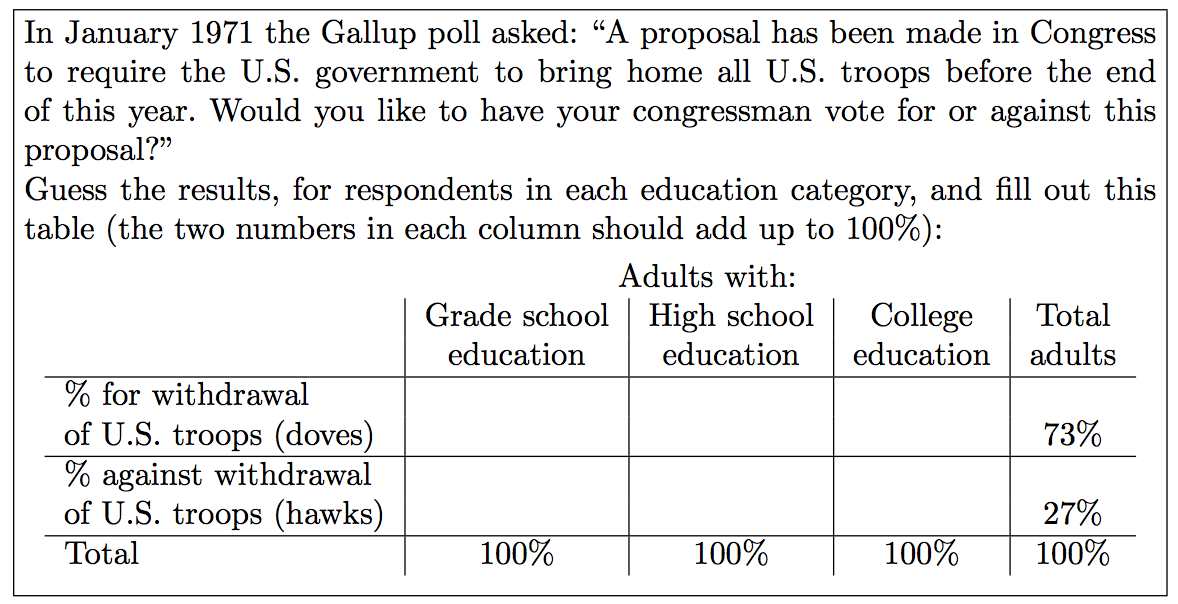
\includegraphics[scale = 0.27]{./images/vietnam_question}
\end{center}



\end{frame}

%%%%%%%%%%%%%%%%%%%%%%%%%%%%%%%%%%%%%%%%
\begin{frame}
\frametitle{Who Were the Doves?}
Which group do you think was most strongly \alert{in favor of} the withdrawal of US troops from Vietnam?
\begin{enumerate}[(a)]
	\item Adults with only a Grade School Education
	\item Adults with a High School Education
	\item Adults with a College Education
\end{enumerate}

\end{frame}
%%%%%%%%%%%%%%%%%%%%%%%%%%%%%%%%%%%%%%%%

\begin{frame}
\frametitle{Who Were the Hawks?}
Which group do you think was most strongly \alert{opposed to} the withdrawal of US troops from Vietnam?
\begin{enumerate}[(a)]
	\item Adults with only a Grade School Education
	\item Adults with a High School Education
	\item Adults with a College Education
\end{enumerate}

\end{frame}
%%%%%%%%%%%%%%%%%%%%%%%%%%%%%%%%%%%%%%%%
\begin{frame}
\frametitle{From The Economist --``Lexington,'' October 4th, 2001}
\begin{quote}
 ``Back in the Vietnam days, the anti-war movement spread from the intelligentsia into the rest of the population, eventually paralyzing the country's will to fight.''
\end{quote}

\end{frame}

%%%%%%%%%%%%%%%%%%%%%%%%%%%%%%%%%%%%%%%%

\begin{frame}
\frametitle{Who \emph{Really} Supported the Vietnam War}
\framesubtitle{Gallup Poll, January 1971}
\begin{center}
\fbox{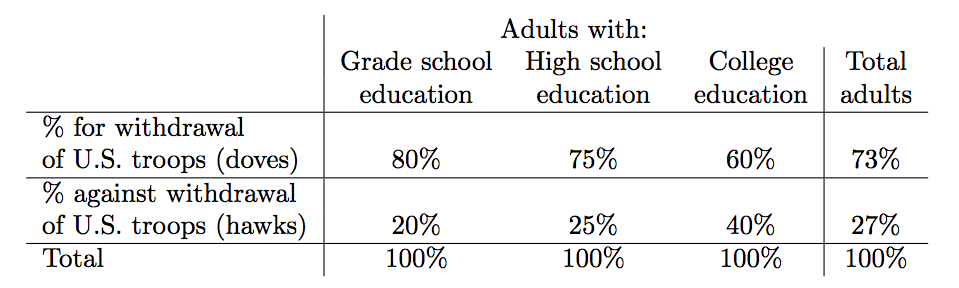
\includegraphics[scale = 0.32]{./images/vietnam_actual}}
\end{center}

\end{frame}
%%%%%%%%%%%%%%%%%%%%%%%%%%%%%%%%%%%%%%%%
\begin{frame}
\begin{center}
 \Huge What about numeric data?
\end{center}
\end{frame}
%%%%%%%%%%%%%%%%%%%%%%%%%%%%%%%%%%%%%%%%
\begin{frame}
\frametitle{Covariance and Correlation: Linear Dependence Measures}

\begin{block}{Two Samples of Numeric Data}
$x_1, \hdots, x_n$ and $y_1, \hdots, y_n$
\end{block}

\begin{block}{Dependence}
Do $x$ and $y$ both tend to be large (or small) at the same time?
\end{block}


\begin{block}{Key Point}
Use the idea of centering and standardizing to decide what ``big'' or ``small'' means in this context.
\end{block}

\end{frame}
%%%%%%%%%%%%%%%%%%%%%%%%%%%%%%%%%%%%%%%%
\begin{frame}
\frametitle{Notation}

	\begin{eqnarray*}
		\bar{x} &=& \frac{1}{n} \sum_{i=1}^n x_i\\
		\bar{y} &=& \frac{1}{n} \sum_{i=1}^n y_i\\
		s_x &=& \sqrt{\frac{1}{n-1} \sum_{i=1}^n (x_i-\bar{x})^2}\\
		s_y &=& \sqrt{\frac{1}{n-1} \sum_{i=1}^n (y_i-\bar{y})^2}
	\end{eqnarray*}

\end{frame}
%%%%%%%%%%%%%%%%%%%%%%%%%%%%%%%%%%%%%%%%
\begin{frame}
\frametitle{Covariance}
	$$s_{xy} = \frac{1}{n-1} \sum_{i=1}^n (x_i -\bar{x})(y_i - \bar{y})$$

\begin{itemize}
	\item Centers each observation around its mean and multiplies.
	\item Zero $\Rightarrow$ no linear dependence
	\item Positive $\Rightarrow$ positive linear dependence
	\item Negative $\Rightarrow$ negative linear dependence
	\item Population parameter: $\sigma_{xy}$
	\item Units?
\end{itemize}
\end{frame}
%%%%%%%%%%%%%%%%%%%%%%%%%%%%%%%%%%%%%%%%
\begin{frame}
\frametitle{Correlation}
	$$r_{xy} = \frac{1}{n-1} \sum_{i=1}^n \left(\frac{x_i -\bar{x}}{s_x}\right)\left(\frac{y_i - \bar{y}}{s_y}\right) = \frac{s_{xy}}{s_x s_y}$$

\begin{itemize}
	\item Centers \emph{and} standardizes each observation 
	\item Bounded between -1 and 1
	\item Zero $\Rightarrow$ no linear dependence
	\item Positive $\Rightarrow$ positive linear dependence
	\item Negative $\Rightarrow$ negative linear dependence
	\item Population parameter: $\rho_{xy}$
	\item Unitless
\end{itemize}
\end{frame}
%%%%%%%%%%%%%%%%%%%%%%%%%%%%%%%%%%%%%%%%
\begin{frame}
\Large \alert{We'll have more to say about correlation and covariance when we discuss linear regression.}
\end{frame}

%%%%%%%%%%%%%%%%%%%%%%%%%%%%%%%%%%%%%%%%
\begin{frame}

\frametitle{Essential Distinction: Parameter vs.\ Statistic}
\framesubtitle{And Population vs.\ Sample}
$N$ individuals in the Population, $n$ individuals in the Sample:

\vspace{1em}
\small
\begin{tabular}{l|l|l}
	&\textbf{Parameter} (Population)&\textbf{Statistic} (Sample)\\
	\hline
	Mean&$\displaystyle\mu_x = \frac{1}{N} \sum_{i=1}^N x_i$& $\displaystyle\bar{x} = \frac{1}{n} \sum_{i=1}^n x_i$ \\
	Var.\ &$\displaystyle \sigma_x^2 = \frac{1}{N}\sum_{i=1}^N (x_i - \mu)^2$ &$\displaystyle s_x^2 = \frac{1}{n-1}\sum_{i=1}^n(x_i - \bar{x})^2$\\
	S.D.\ &$\sigma_x = \sqrt{\sigma_x^2}$ &$s_x = \sqrt{s^2}$ \\
	&&\\
	\hline
	&&\\
	\alert{Cov.\ }&\alert{$\displaystyle \sigma_{xy} = \frac{\sum_{i=1}^N(x_i - \mu_x)(y_i - \mu_y)}{N}$} &\alert{$\displaystyle s_{xy} = \frac{\sum_{i=1}^n(x_i - \bar{x})(y_i - \bar{y})}{n-1}$}\\
	\alert{Corr.\ } & \alert{$\displaystyle \rho = \frac{\sigma_{xy}}{\sigma_x \sigma_y}$}& \alert{$\displaystyle r = \frac{s_{xy}}{s_x s_y}$}
\end{tabular}

\end{frame}

\begin{frame}
  \frametitle{Next Up: Basic Probability}
  %\begin{enumerate}
    %\item Complete the ``Odd Questions'' quiz posted on Piazza \texttt{OddQuestions.pdf} -- we'll be discussing these in class.
     % \vspace{1em}
%    \item 
    If you're rusty on permutations, combinations, etc. from High School math, read ClassicalProbability.pdf on the webpage.
  %\end{enumerate}
\end{frame}
%%%%%%%%%%%%%%%%%%%%%%%%%%%%%%%%%%%%%%%%
\end{document}
